\section{Object Reconstruction}
\subsection{Tracks}

Building a track, which represents the three dimensional path of the a charge particle, begins with forming hits in both the SMT and CFT tracking detectors. An SMT hit cluster is formed when a group of adjacent silicon strips register enough charge generated from an ionizing charged particle traversing the detector. The presence of the magnetic field in the SMT causes the electron-hole pairs to drift at an angle, known as the Lorentz angle. This drift angle is corrected for when determining the center of the silicon strip. The center of the hit cluster is formed by the charge weighted average of the centers of each silicon strip. The fine granularity of the SMT silicon strips allows an $x$-$y$-$z$ coordinate measurement for each hit in the detector. The axial resolution of an SMT hit is $10~\mu m$ and the $z$ coordinate resolution is $35~\mu m$. A hit in the CFT is formed when the two fibers in each layer register scintillation light indicating the presence of the charge particle traversing the fibers. The $x$-$y$ position of the hit can be measured because each fiber layers is rotated by $3^{\circ}$~with respect to the beam axis. The $z$ hit position is inferred from the $x$-$y$ coordinate measurement and the fibers which produced the signal. 
The axial resolution of a CFT hit is $100~\mu m$ and the $z$ coordinate resolution $2$~cm.

A track formed by pattern recognition software that takes SMT and CFT hit clusters as input to form a path in three dimensions, which represents the path of the charged particle. Because the tracking detectors are immersed in a $2$T magnetic field, the paths of the charged particles with be a three-dimensional helix as opposed to a straight line in absence of the magnetic field. The goal of the track finding algorithms is to combine SMT and CFT hits into possible track candidates and determine the parameters which fully define the track helix. There are two track finding algorithms employed in the $\dzero$~event reconstruction software. The first algorithm uses a histogramming technique to find finds and the second algorithm uses a road method technique. These two techniques are described in more detail below. A global track reconstruction algorithm combines the output of the two algorithms to create a final set of reconstructed tracks.

\subsubsection{Histogramming Tracking Finding Method (HTF)}
\label{htf}
The histogramming method works by taking a list of hits in the SMT and CFT and transforming their coordinates transverse coordinates (x,y) into the ($\rho$,$\phi$) plane, where $\rho$ is the track curvature and $\phi$ is the azimuthal angle. The conversion to the new unit is done by a Hough transformation. Hits resulting from the same charged particle and thus the same track parameters will form a peak in this plane. The height of the peak will be $n(n-1)/2$, where $n$~is the number hits. This new histogram then goes through a cleaning procedure, called a 2D Kalman filter, which for the first time includes material related affects such as multiple scattering and energy loss. The Kalman filter has several tunable parameters such as the maximum $\chi^{2}$ of the track fit and the minimum number is SMT and CFT hits. The result of the filter is to have at most one $r$-$\phi$ hit in each layer and modified track parameters. The $z$~coordinate information is included by creating a new histogram in $(r,z)$ and performing a Hough transformation to the $(z_{0},C)$ plane, where $z_{0}$ is the position of the track along the origin and $C$ is the track inclination defined as $C = \frac{dr}{dz}$. Finally, the tracks are extrapolated either inward toward the SMT if the track finding began in the CFT or outward toward the CFT if the track finding began in the inner SMT detector. The histogramming method has advantages over titional road finding algorithms because it does not need to compute all possible combinations of tracks, which grows exponentially with increasing luminosity. The method is also well suited to detectors without distinct layers such as the SMT detector.


\subsubsection{Alternative Algorithm Tracking (AA)}
\label{aa}
The alternative algorithm tracking method works by building a seed track in one layer and building a track by incrementally including more layers of the SMT and CFT detectors. The algorithm begins by taking SMT clusters in the innermost layers and adding additional layers if the axial angle between the next point and the beam spot is less than a certain tunable value. Additional layers are included if the previous condition is true and also if the resulting ius of curvature of the track hypothesis is greater than $30$~cm, which indicates the track must have $p_{T}>180$~MeV. The new track must also have a track fit $\chi^{2}<16$. All possible combinations that meet these requirements are kept in the tracking algorithm for later filtering. The algorithm also allows for missing hits in the SMT or CFT by re-defining the track if a hit in one of the outer layers is consistent with a previously defined track. The number of such missing hits is a tunable parameter in the algorithm. AA tracking also allows for so-called CFT-only tracks built from seeds in the CFT detector that have less than 3 hits in the SMT detector. Allowing tracks to be built in this manner dramatically increases the overall efficiency of the algorithm. The final step in the algorithm is to remove overlapping tracks by selecting the track with the lowest $\chi^{2}$.


\subsection{Primary Interaction Vertex}
\label{pvreco}
The primary hard scatter interaction vertex is very important to locate in to allow discrimination of physics objects resulting from the $\ppbar$~collision and objects created from noise in the detector or other low energy inelastic $\ppbar$~collisions. The primary vertex is defined as the three-dimensional position of the hard-scatter interaction. These vertices are found using the adaptive primary vertex algorithm. The algorithm begins by attempting to assign all tracks with $p_{T}>0.5$~GeV and at least two SMT hits to a vertex where the track paths intersect. The result of this first pass fit to the primary vertex is a $\chi^{2}$ for each track. The algorithm then attempts a second path fit to the primary vertex except this time each track receives a weight, shown in Eq.~\ref{pvweight}, that is contains to the $\chi^{2}$ of the previous fit.

\begin{equation}
\label{pvweight}
w_{i} = \frac{1}{1+e^{(\chi^{2}_{i} - \chi^{2}_{\rm{cutoff}})/2T}}
\end{equation}

The parameters $\chi^{2}_{\rm{cutoff}}$ and T are input parameters to the algorithm and have similar interpretations to the chemical potential and temperature in Fermi statistics. If the weight of the track is less than $10^{-6}$ the track is not included in the next round of fitting. This procedure is repeated until the difference of weights from the previous iteration for each track is less than $10^{-4}$.

The adaptive vertexing algorithm produces a list of possible vertices of which one might be the hard scatter vertex. To determine the hard scatter vertex a minimum bias~\footnote{A minimum bias vertex is a vertex from an inelastic $\ppbar$~collision.} vertex probability is calculated. The probability, shown in Fig~\ref{minbias} peaks at zero for the hard-scatter vertex and is uniform for inelastic $\ppbar$~collision vertices. The vertex used as hard-scatter vertex in an event is the one that has the lowest minimum bias probability. Finally, the vertex resolution of the algorithm for events with no heavy flavor production is 9.3 $\mu$m and 12.8 $\mu$m for events with heavy flavor.

\begin{figure}[!h!tbp]
\begin{center}
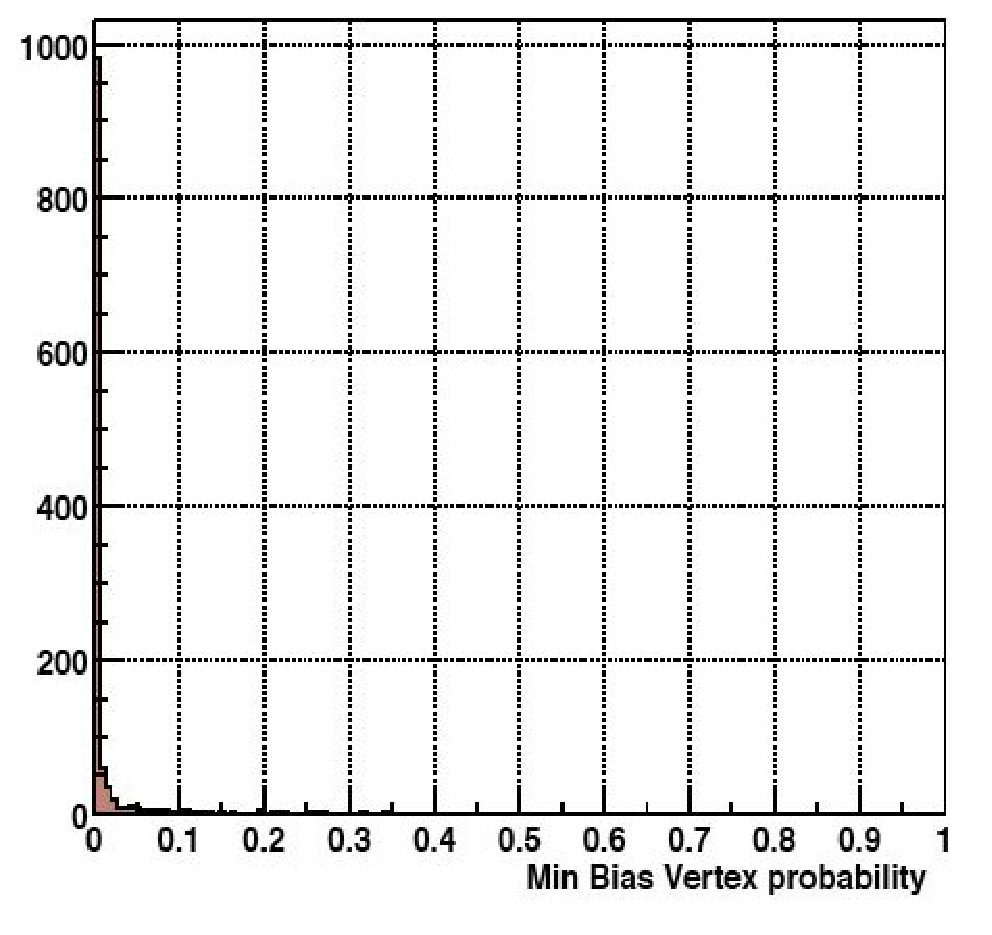
\includegraphics[width=0.45\textwidth]{eps/Reco/MBP_PV.eps}
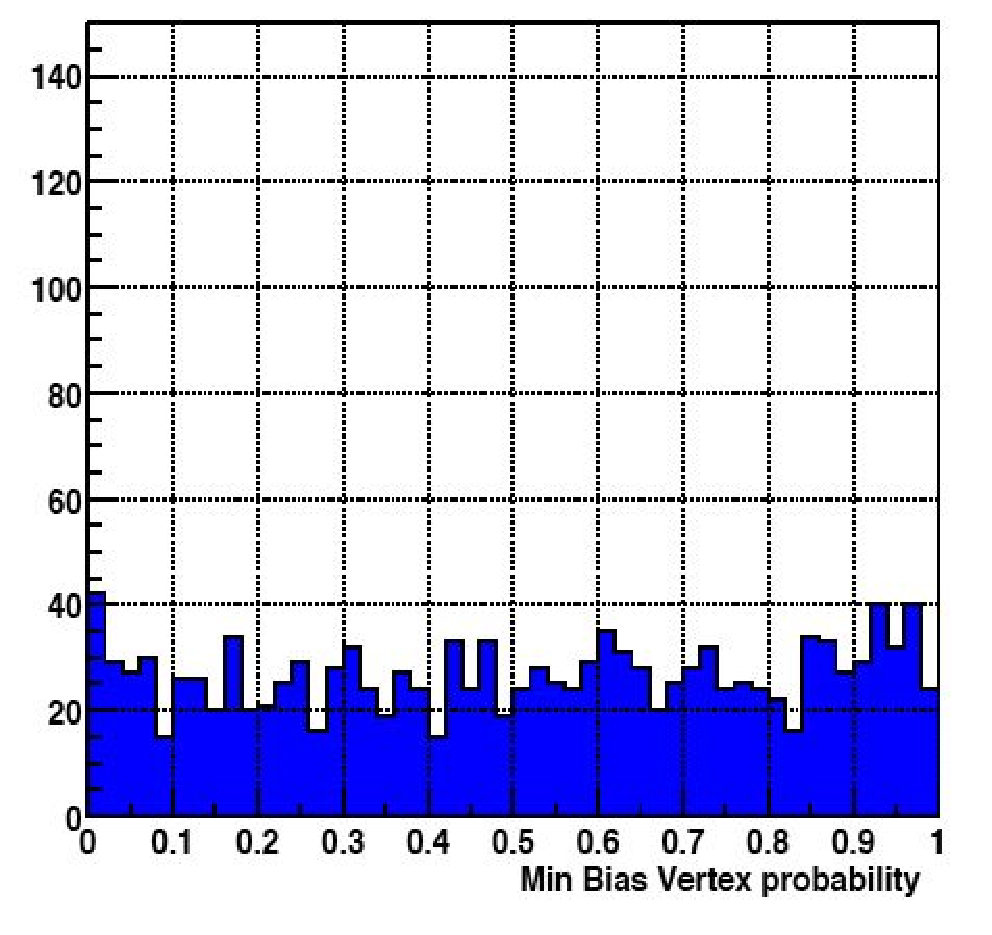
\includegraphics[width=0.45\textwidth]{eps/Reco/MBP_MB.eps}
\end{center}
\vspace{-0.1in}
\caption[minbias]{Minimum bias probability for the hard-scatter vertex (left) and inelastic $\ppbar$ vertices (right).}
\label{minbias}
\end{figure}


\subsection{Electrons}
Electrons are characterized by narrow electromagnetic showers produced in the electromagnetic calorimeter. Electrons are first identified by searching for a cluster of EM calorimeter towers with energies above a given threshold value. Once a tower is found above threshold the electron candidate is defined as the towers surrounded the highest $E_{T}$ tower in a cone of ius 0.4. Since electrons are light they will deposit almost all of their energy in the first few layers of the electromagnetic calorimeter. Once the electron candidate is found it is required to have at least $90\%$ of it's energy deposited in this region. The shape of the electromagnetic shower induced by the depleted uranium should also be consistent with an electron or photon. The shower shape is fit to the expected shower shape determined from simulation and the resulting $\chi^{2}$ must be less than 50. To remove photons, which will produce similar deposits of energy and shower shapes, the electromagnetic cluster is required to be matched to a track found by the global track reconstruction algorithm. The matched track is then required to have $p_{T}>5$~GeV. To ensure that the electron is well measured it is also required to be narrow and isolated from other electromagnetic clusters. The isolation, defined in Eq.~\ref{fiso}, is required to be less than 0.15

\begin{equation}
\label{fiso}
\rm{f_{iso}} = \frac{E_{tot}(\Delta R <  0.4) - E_{EM}(\Delta R <  0.2)}{E_{EM}(\Delta R <  0.2)}
\end{equation}

Finally to ensure high quality electrons, likelihood discriminant is created using seven variables that will separate electrons from W/Z boson decays from jets with large electromagnetic fractions (fake electrons). Electrons with a likelihood discriminant greater than 0.85 are considered true electrons from a W/Z decay.

\subsection{Muons}
\label{muonreco}
Muon are reconstructed by requiring hits in the layers of the muon system from both the scintillators and the wire chambers. Muons are required to register at least two wire hits and at least one scintillator hit in the A layer. If this condition is met, the muon is required to have at least two wire hits in the B and C layers as well as at least one scintillator hit in this region. By requiring hits in all three layers it is possible to construct a local momentum measurement due to the curvature induced by the toroid magnet; however, typically the resolution of this measurement is quite poor. To improve the resolution, the local muon track is required to be matched to a track found by the global track reconstruction algorithm. The track is required to be $\Delta R<0.5$~from the local muon track. To remove muons produced by cosmic rays the muon is required to arrive at the three muon layers less than $10$~ns after the bunch crossing. To further reduce the cosmic ray background the muon track is required to originate from the primary vertex. The ensure this requirement the muon track must have a transverse distance of closest approach (DCA) less than 0.2 cm if there are no SMT hits and less than 0.02 cm if there is at least one SMT hit for the track. The track is also required to be within 1 cm of the primary vertex in the $z$ direction. The final background contamination to remove are muons from heavy flavor decays (e.g. $B \rightarrow \mu\nu_{\mu} D$). These muons tend to be embedded inside or nearby a jet since they are decay product of the boosted mesons that makeup the jet. To remove this background muons are required to be isolated ($\Delta R(\mu,\rm{jet}) > 0.5$)~from nearby jets. Also, a muon track isolation variable, defined in Eq.~\ref{trackiso}, is required to be less than 0.2. 

\begin{equation}
\label{trackiso}
\frac{1}{p_{T}(\mu)} \times \sum_{\rm{tracks \neq muon~ \Delta R < 0.5 }}p_{T}(\rm{track})
\end{equation}

A similar variable for calorimeter tower energies, shown in Eq.~\ref{caliso}, is also required to be less than 0.2.

\begin{equation}
\label{caliso}
\frac{1}{p_{T}(\mu)} \times \sum_{\rm{cal~tower~0.1 < \Delta R < 0.4 }}E_{T}(\rm{cal~tower})
\end{equation}

Muons that satisfy all of these criteria are considered true muons from a W/Z decay.


\subsection{Jets}
\label{jetreco}
A jet is the result of an strong interaction particle, such as a quark or gluon, that hadronizes producing a collection of collimated hadrons traveling in the same direction as the origination parton~\footnote{A parton is a fundamental particle such as a quark or a gluon that is a constituent of a hadron.}. The Run II improved legacy cone algorithm~\cite{Blazey:2000qt} is used to reconstruct jets in the $\dzero$~calorimeter. This algorithm starts with calorimeter towers with transverse energies~\footnote{The transverse energy is the energy of the calorimeter tower weighted by the sine of the polar angle $\theta$ of the tower. $E_{T} = E \times \sin(\theta)$.} greater than $0.5$~GeV and uses them as seeds around which the jet is built. If there is greater than $1$~GeV is total transverse energy in a cone ius if $0.5$ in $y-\phi$~space~\footnote{$y$~is the rapidity of the jet.}, then the collection of towers is considered a jet. The center of the jet is defined by the $E_{T}$ weighted midpoint of each calorimeter tower. If the cone axis of the jet is different from the previous iteration, a new jet is formed and the total $E_{T}$ is again calculated. This process is repeated until a stable jet is found. The result of this process is a list of stable jets with well-defined transverse energy $E_{T}$, rapidity $y$, and, azimuthal angle $\phi$. The final step of the jet finding algorithm is to remove overlapping (duplicate) jets and either split large jets or merge nearby jets. Two overlapping jets are merged if they contain more than half of each others energy in their own jets. If the overlapping jets are not merged, then they are split into two distinct jets whose total $E_{T}$ and cone axis are then recomputed.

Cone jets have several advantages both experimentally and theoretically. Since the jets are defined by rapidity and $\phi$, they are invariant under boosts along the longitudinal direction (beam axis). This is important because the longitudinal boost of the event will typically be large with resepect to the $\ppbar$~rest frame. The other advantage of cone jets is they are infrared safe meaning that one can calculate jet properties in the low energy regime of a theory without incurring singularities.

Once the final list of jets has been created, the final step is to impose a set of quality criteria that will help remove fake jets created out of calorimeter noise and remove electromagnetic particles such as electrons and photons. To remove jets created by electromagnetic particles a jet is require to have between 5 and 95$\%$ of it's energy deposited in the hadronic calorimeter because electrons and photons tend to deposit almost all of their energy in the electromagnetic calorimeter. Also, a jet is required to be isolated ($\Delta R>0.5$) from all electromagnetic clusters in the detector. To remove fake jets created by calorimeter noise, the jet is required to have at least 60$\%$ of it's energy deposited in the fine hadronic calorimeter since this detector gives significantly better energy measurements compared to the coarse hadronic calorimeter. To remove jets created by a single noisy tower all jets are required to have at least two or more calorimeter cells containing at least $90\%$ if the jet energy. Also, the ratio of the most energetic tower to the second most energetic tower must be less than 10. 

\subsection{Missing $E_{T}$}
Missing transverse energy, $\met$, is a useful quantity to calculate because it is highly correlated with the energy an undetected neutrino carries away from the events. The missing energy is only calculated in the transverse plane (x-y) because there is no net momentum in this plane since the collision only occurs along the beam axis. The total missing energy of the event can not be calculated however because of the unknown boost along the longitudinal direction from the hard scatter process.  The $\met$~is formed by summing all calorimeter cells in the electromagnetic and fine hadronic calorimeters and then balanced so there is no net transverse momentum in the event. The $\met$ is further corrected for high $p_{T}$ leptons in the event. The total $\met$ is defined in Eq.~\ref{met}.

\begin{equation}
\label{met}
\left[~\sum_{\rm{cells}} E_{T}~\right]+ p_{T}(\ell) + \rm{ME}_{T} = 0
\end{equation}

\subsection{$B$-Jets}
\label{bidreco}
Events with heavy flavor jets (jets formed from initial $b$ or $c$ quarks) are important to measure because many fundamental particles, such as the top quark, will decay into a $b$ quark leaving it as one of the few signatures of it's existence. Jets formed from $b$ quarks are unique from other jets produced from light quarks because the $B$~meson (a combination of a $b$ quark and a light quark) has a much longer lifetime than lighter mesons. The result of this long lifetime is a displaced decay vertex from the primary interaction vertex. The typical decay length, which is the distance from the decay vertex from the primary vertex, is $\sim$few mm. The goal of the $B$-jet finding algorithm is to use this information and more to identify heavy flavor jets from ordinary light flavor jets.

The $B$-jet selection algorithm at $\dzero$~uses a neural network (NN) to separate events with heavy flavor (B,D mesons) from light flavor events. The neural network is trained on seven variables that show discrimination between heavy and light flavor events. The seven variables are shown in Table~\ref{nnvars}. The neural network takes as input good quality jets and the tracks which point towards those jets. All jets must have at least two associated tracks with $p_{T}>1$~GeV. Jets that fail these criteria are considered light jets. The network was trained with $Z\rightarrow b\bar{b}$ and direct QCD $b\bar{b}$ production as heavy flavor signal-like events and $Z\rightarrow q\bar{q}$ and QCD $q\bar{q}$ production as light flavor background-like events. The output of the neural network is new probabilistic variable which peaks at 1 for jets with heavy flavor and 0 for light flavor jets. A jet is considered a $B$-jet if the NN value is greater than 0.775. For this choice of NN cut, the average $b$-tagging efficiency for central jets is $47\%$ and a light jet mis-tag rate of $0.47\%$.

\begin{table}[!h!tbp]
\begin{center}
\begin{tabular}{c|c}
\multicolumn{2}{c}
{\underline{Variables Used in $B$-jet Neural Network}} \\
Rank	&	Variable Description	\\
\hline
1		&	Decay length significance ($\frac{L_{T}}{\delta L_{T}}$) of the displaced vertex	\\
2		&	Weighed combination of the input tracks' impact parameter significance ($\frac{IP}{\delta IP}$)	\\
3		&	Probability that the jet originates from the primary interaction vertex	\\
4		&	$\chi^{2}$/N$_{dof}$ of the displaced vertex fit	\\
5		&	Number of tracks used to reconstruct the displaced vertex	\\
6		&	Mass of the tracks used to reconstruct the displaced vertex	\\
7		&	Number of displaced vertices found inside the input jets		\\
\end{tabular}
\vspace{-0.1 in}
\caption[nnvars]{Variables used in the neural networks training. The variables are listed in order of relative importance as determined in the training.}
\label{nnvars}
\end{center}
\end{table} 